\documentclass[../main/main.tex]{subfiles}
\begin{document}

\chapter{Gravitation}

\section{The action in the curved space}

\textsf{Carroll, sec. 4.3}\\

Now we can obtain well defined actions for various kinds of matter fields $\Phi$ as follows \footnote{We use the compact notation $\sqrt{-g}:=\sqrt{-\det g}$.}
\[S_\Phi=\int_M\diff4x\sqrt{-g}\lag(\Phi,\nabla\Phi)\]
From such action we expect to get fully covariant e.o.m. 

For instance, take the Lagrangian for a real scalar field
\[S_\phi=\int\diff4x\sqrt{-g}\left[-\frac12\cde\mu\phi\nabla^\mu\phi-V(\phi)\right]\]
If we use the least action principle in order to obtain the e.o.m. we obtain for a fixed $\delta\phi$:
\begin{align*}
\delta S_\phi
&=\int\diff4x\sqrt{-g}\p{-\cde\mu\delta\phi\nabla^\mu\phi-\delta\phi\pder V\phi}\\
&=\int\diff4x\sqrt{-g}\p{\cde\mu\nabla^\mu\phi-\pder V\phi}
\end{align*}
and imposing this to be zero we obtain the e.o.m. for a real scalar field
\begin{equation}\boxed{
\nabla_\mu\nabla^\mu\phi=\pder V\phi
}\end{equation}
which is a fully covariant equation. 

For the EM field we obtain
\[S_A=\int\diff4x\sqrt{-g}\p{-\frac14F_{\mu\nu}F^{\mu\nu}+A_\mu J^\mu}\qquad\text{with}\qquad F_{\mu\nu}=\cde\mu A_\nu-\cde\nu A_\mu\]
and for a fixed $\delta A_\mu$ we have
\begin{align*}
\delta S_A&=\int\diff4x\sqrt{-g}\left[-\p{\cde\mu\delta A_\nu}F^{\mu\nu}+\delta A_\mu J^\mu\right]\\
&=-\underbrace{\int\de4x\sqrt{-g}\cde\mu(\delta A_\nu F^{\mu\nu})}_{\int\diff4x\pde\mu\p{\sqrt{-g}\delta A_\nu F^{\mu\nu}}=0}+\int\diff4x\sqrt{-g}\delta A_\nu\p{\cde\mu F^{\mu\nu}-J^\nu}
\end{align*}
hence we obtain the e.o.m.
\begin{equation}\boxed{
\cde\mu F^{\mu\nu}=J^\nu\qquad\Rightarrow\qquad\cde\mu J^\mu=0
}\end{equation}
where the relation on the r.h.s. is given by properties of $F^{\mu\nu}=0$. Again, these e.o.m. are fully covariant. 

Clearly, these e.o.m.'s (approximately) reduce to the special relativistic ones by restricting to LIFs e.g. normal coordinates) $\hat x^\alpha$ in which $\Gamma\simeq0$. They provides an explicit realization of the EEP and describe how the dynamics of matter field are affected by a non-trivial gravitational field. 

\subsection{Einstein-Hilbert action}

\textsf{Carroll, sec. 4.2-4.3}\\

So far the metric has been considered non-dynamical, realizing the EEP. We now face the opposite problem:
\begin{enumerate}[label=\textbullet]
\item What are the e.o.m. of the metric?
\item How is it affected by matter and gauge fields?
\end{enumerate}

We will not follow a historical path, but again invoke the \emph{least action principle}. In fact, the matter and gauge Lagrangians $\lag(\Phi,\nabla\Phi)$ discussed above already contain interaction terms between gauga/matter fields and the metric. 

We can however wonder whether there can be purely gravitational terms. In particular, we should look for a coordinate-independent 2-derivative action:
\[\int\diff4x\sqrt{-g}\lag_G(x)\]

So the question is:
\begin{enumerate}[label=\textbullet]
\item Which 2-derivatives scalar Lagrangians $\lag_G(x)$ can we construct out of $\met\mu\nu$?
\end{enumerate}
There is only one possibility: $\lag_G\propto R$. It is then natural to include in the action the \textbf{Einstein-Hilbert term}:
\[S_{\text{EH}}[g]=\frac1{2\kappa}\int\diff4x\sqrt{-g}R\]

Notice that $[R]=L^{-2}$, $[\diff4x\sqrt{-g}]=L^4$, $[S]=ET$ and
\[[\kappa]=\left[\frac{L^2}{ET}\right]=\left[\frac TM\right]=\frac{[G]}{c^3}\]
Indeed we will see that $\kappa\sim\frac{G}{c^3}$.

We are then lead to consider 2-derivative actions of the form 
\[S=S_{\text{EH}}[g]+S_\Phi=\frac1{2\kappa}\int\diff4x\sqrt{-g}R+S_\Phi\]
Extremization with respect to $\Phi$ produces the equations written above. We instead still have to comput the \emph{metric e.o.m.} obtained by extremizing with respect to $\met\mu\nu$. 

We will do this in two steps, described in following section. 

\section{The Einstein equations}

Let's start from the action 
\[S=S_{\text{EH}}[g]+S_\Phi=\frac1{2\kappa}\int\diff4x\sqrt{-g}R+S_\Phi\]

\subsubsection{a) Variation of $S_{\text{EH}}$}

We may extremize with respect to $\delta\met\mu\nu$. However this is completely equivaent to extremizing with respect to to $\delta\imet\mu\nu$ since
\[\imet\mu\nu\met\nu\rho=\delta^\mu_\rho\qquad\Rightarrow\qquad\delta\imet\mu\nu\met\nu\rho+\imet\mu\nu\delta\met\nu\rho=0\]
implies
\begin{equation}\boxed{
\delta\imet\mu\nu=-\delta\met\rho\sigma\imet\rho\mu\imet\sigma\nu
}\end{equation}
hence $\delta\met\mu\nu$ and $\delta\imet\mu\nu$ are in one-to-one correspondence. 

We get two contributions
\[\delta\int\diff4x\sqrt{-g}R=\delta\int\diff4x\sqrt{-g}\imet\mu\nu\ricc\mu\nu=\int\diff4x\big(\underbrace{\delta\sqrt{-g}}_{\circled1}R+\sqrt{-g}\delta\imet\mu\nu\ricc\mu\nu+\sqrt{-g}\underbrace{\imet\mu\nu\delta\ricc\mu\nu}_{\circled2}\big)\]

Let's rewrite $\circled1$ and $\circled2$. 
For $\circled1$ we observe that ($g=\met\mu\nu$)
\begin{equation}\boxed{
\log(\det g)=\Tr(\log g)
}\end{equation}
indeed $\det g=\prod_a\lambda_a$ and $\Tr(\log g)=\sum_a\log \lambda_a$ . Then
\begin{align*}
\delta\det g&=\delta e^{\log(\det g)}=\delta e^{\Tr\log g}=e^{\Tr\log g}\Tr(\delta\log g)\\
&=(\det g)\Tr\inv g\delta g=(\det g)\imet\mu\nu\delta\met\mu\nu=-(\det g)\delta\imet\mu\nu\met\mu\nu
\end{align*}
But $\delta\sqrt{-g}=-\frac1{2\sqrt{-g}}\delta\det g$ and so
\begin{equation}\boxed{
\delta\sqrt{-g}=-\frac12\sqrt{-g}\delta\imet\mu\nu\met\mu\nu
}\end{equation}

For $\circled2$ since $\delta\ricc\mu\nu=\delta\curv\rho\mu\rho\nu$ we have
\begin{align*}
\delta\curv\rho\mu\sigma\nu&=\delta[\pde\sigma\chris\rho\mu\nu+\chris\rho\lambda\sigma\chris\lambda\mu\nu-(\sigma\leftrightarrow\nu)]\\
&=\pde\delta\chris\rho\mu\nu+\delta\chris\rho\lambda\sigma\chris\lambda\mu\nu+\chris\rho\lambda\sigma\delta\chris\lambda\mu\nu-\pde\nu\delta\chris\rho\mu\sigma-\delta\chris\rho\lambda\nu\chris\lambda\mu\sigma-\chris\rho\lambda\nu\delta\chris\lambda\mu\sigma
\end{align*}
Recall that $\delta\chris\mu\nu\rho$ is a tensor
\[\cde\sigma\delta\chris\rho\mu\nu=\pde\sigma\delta\chris\rho\mu\nu+\chris\rho\lambda\sigma\delta\chris\lambda\mu\nu-\chris\lambda\mu\sigma\delta\chris\rho\lambda\nu-\chris\lambda\nu\sigma\delta\chris\rho\mu\lambda\]
And using the latter and the corresponding equation for $\nu\leftrightarrow\sigma$ we obtain
\[\delta\curv\rho\mu\sigma\nu=\cde\sigma\delta\chris\rho\mu\nu-\cde\nu\delta\chris\rho\mu\sigma\]
which implies
\[\delta\ricc\mu\nu=\cde\rho\delta\chris\rho\mu\nu-\cde\nu\delta\chris\sigma\mu\sigma\]
and
\[\imet\mu\nu\delta\ricc\mu\nu=\cde\rho\p{\imet\mu\nu\delta\chris\rho\mu\nu-\imet\rho\mu\delta\chris\sigma\mu\sigma}\equiv\cde\rho\delta V^\rho\]

Thanks to the results of sec.~\ref{sec:integr-curv-space} we can write the result in the form of a covariant derivative whose integration vanishes because of vanishing boundary terms
\[\int\diff4x\sqrt{-g}\cde\rho\delta V^\rho\equiv\int\diff4x\pde\rho\p{\sqrt{-g}\delta V^\rho}=0\]

Putting these results together, we then arrive at the conclusion that 
\begin{equation}\boxed{\begin{split}
\delta S_{\text{EH}}&=\frac1{2\kappa}\int\diff4x\sqrt{-g}\delta\imet\mu\nu\p{\ricc\mu\nu-\frac12\met\mu\nu R}\\
&\equiv\frac1{2\kappa}\int\diff4x\sqrt{-g}\delta\imet\mu\nu\eten\mu\nu
\end{split}}\end{equation}
where we used the definition of the Einstein tensor $\eten\mu\nu=\ricc\mu\nu-\frac12\met\mu\nu R$. 

\subsubsection{b) Variation of $S_\Phi$}

In general we simply define the \textbf{energy-momentum} tensor (or \textbf{stress-energy} tensor) $\emt\mu\nu$ by
\begin{equation}\boxed{
\delta S_{\Phi}=-\frac12\int\diff4x\sqrt{-g}\delta\imet\mu\nu\emt\mu\nu\equiv\frac12\int\diff4x\sqrt{-g}\delta\met\mu\nu\iemt\mu\nu
}\end{equation}
Notice that, by definition, $\emt\mu\nu$ is \emph{symmetric}
\begin{equation}\boxed{
\emt\mu\nu=\emt\nu\mu
}\end{equation}

It does not always coincides with the ``canonical'' $\temt\mu\nu$ but Belifante showed that one can ``improve'' $\temt\mu\nu$ to get $\tiemt\mu\nu$ to get $\iemt\mu\nu$. 

Then the application of the least action principle $\delta S=\delta S_{\text{EH}}+\delta S_\Phi=0$ leads to the \textbf{Einstein equations} (EE)
\begin{equation}\boxed{
\eten\mu\nu=\kappa\emt\mu\nu
}\end{equation}

Notice that $\icde\mu\eten\mu\nu=0$ implies
\begin{equation}\boxed{
\icde\mu\emt\mu\nu=0
}\end{equation}

%%%%%%%%%%%%LECTURE 11%%%%%%%%%%%%%%

\section{The energy-momentum tensor}

\textsf{Carroll, sec. 1.9-1.10}\\

Let's analyze the energy momentum tensor $\emt\mu\nu$ in order to understand its meaning and properties. 

Consider the Minkowski spacetime, we have
\begin{equation}\label{eq:cov_der_iemt_vanish}\boxed{
P^\mu=\int\diff3x\iemt0\mu(x)\qquad\Rightarrow\qquad E=\int\diff3x\iemt00\qquad P^i=\int\diff3x\iemt0i
}\end{equation}
hence $\iemt00(x)$ and $\iemt0i(x)$ should be meant respectively as ``energy density'' and ``(linear) momentum density''. 

On the other side, the interpretation of $\iemt ij$ requires  more work. Let
\begin{eqalign}
	P_V^j(t) := \int_V \diff3x\iemt0j(x)
\end{eqalign}
then using Stoke's theorem we obtain\footnote{The minus sign introduced is due to $\der{}{t}\iemt0j = - \partial_i\iemt ij$ given by Equation~\eqref{eq:cov_der_iemt_vanish} in the flat metric.}
\begin{eqalign}
	\der{P_V^j}{t} = -\int_V\diff3x\partial_i\iemt ij = - \int_S \diff{}{S_i} \iemt ii =: F_V^j
\end{eqalign}
with $S:=\partial V$ is the boundary of $V$ and $\diff{}{\vec S}$ is the outward pointing surface form on $S$: 
\begin{figure}[H]
\centering
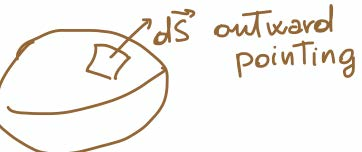
\includegraphics[width=4cm]{../img/surf_form.jpg}
\end{figure}
\noindent
Hence we can interpret the object $F_V^j$ as the \textbf{force exerted on V} and consequently $\iemt ij$ as the force per unit area pushing in the $j$-direction surface portion. For this reason $\iemt ij$ is called \textbf{(3D) stress tensor}. In particular $\iemt ii =: \press$ is the \textbf{pressure}, while $\iemt ij$ for $i\neq j$ are \textbf{shear-terms}.

In more general spacetimes, this interpretation holds only locally and approximately in a LIF (e.g. of normal coordinates).

\subsection{The point particle case}

\newcommand{\Part}{\text{\tiny part}}

In fact, we will see that this is a subtle concept, once one takes into account the particle's backreaction. But let us for the moment ignore these issues. We already know the particle's action:
\begin{eqalign}
	S_\Part &= \frac12\int\diff{}{\lambda} [\inv e\met\mu\nu(X)\dot X^\mu\dot X^\nu - m^2e]\\
	&=\frac12\int\diff{}{\lambda}\int\diff4x\delta^4(x-X(\lambda))[\inv e\met\mu\nu(x)\dot X^\mu\dot X^\nu-m^2e]
\end{eqalign}

Now consider an infinitesimal metric variation $\delta\met\mu\nu$:
\begin{eqalign}
	\delta S_\Part &= \frac12\int\diff4x\delta\met\mu\nu(x)\int\diff{}\lambda\inv e\delta^4(x-X(\lambda))\dot X^\mu\dot X^\nu\\
	&=: \frac12\int\diff4x\sqrt{-g}\,\delta\met\mu\nu\iemt\mu\nu
\end{eqalign}
i.e.
\begin{eqalign}\boxed{
	\iemt\mu\nu_{(\Part)}(x) = \int\diff{}{\lambda}\inv e\dot X^\mu\dot X^\nu \frac{\delta^4(x-X(\lambda))}{\sqrt{-g(x)}}
}\end{eqalign}
where the term $\frac{\delta^4(x-X(\lambda))}{\sqrt{-g(x)}}$ transform as a scalar. 

We can take proper $\lambda$: $e(\lambda) = 1$ so that $\dot X^\mu = P^\mu(\lambda)$ with $P^\mu P_\mu = -m^2$, in this case 
\begin{eqalign}\boxed{
	\iemt\mu\nu_{(\Part)}(x) = \int\diff{}{\lambda}P^\mu(\lambda) P^\nu(\lambda) \frac{\delta^4(x-X(\lambda))}{\sqrt{-g(x)}}
}\end{eqalign}
is covariant.  Furthermore we can rewrite
\begin{eqalign}
	\delta^4(x-X(\lambda)) = \delta(x^0 - X^0(\lambda))\delta^3(\vec x-\vec X(\lambda)) = \frac{\delta(\lambda-\bar\lambda)}{\dot X^0(\bar\lambda)}\delta^3(\vec x-\vec X(x^0)) = \frac{\delta(\lambda-\lambda_0)}{P^0(x^0)}\delta^3(\vec x-\vec X(x^0))
\end{eqalign}
where in the last step we assumed $\dot X^0>0$: 
\begin{figure}[H]
\centering
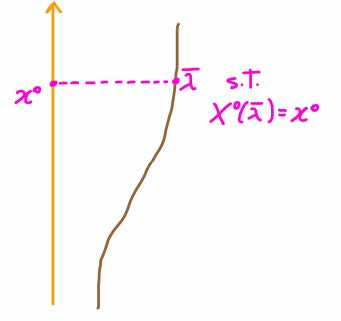
\includegraphics[width=4cm]{../img/delta_rewr_iemt_interp.jpg}
\end{figure}
\noindent
Hence
\begin{eqalign}\boxed{
	\iemt\mu\nu_{(\Part)}(x) =P^\mu(t) P^\nu(t) \frac{\delta^3(\vec x-\vec X(t))}{P^0(t)\sqrt{-g(x, \vec x)}}
}\end{eqalign}
In a LIF $\hat x^\alpha = (\hat x^0, \hat x^a)$ we get
\begin{eqalign}
	\hiemt00 &= \hat P^0\delta^3(\vec x - \vec X(t))\quad\textbf{energy density}\\
	\hiemt0a &= \hat P^a\delta^3(\vec x - \vec X(t))\quad\textbf{momentum density}
\end{eqalign}

\subsection{Perfect fluids}

At large enough distances, many macroscopic systems can be approximated as \textbf{perfect fluids}, that is, such that any observer solidal with any fluid element, sees the fluid around him as isotropic. This happens if the free path of the interacting particles is much shorter than the relevant length scales. 

In the rest LIF $\hat x^\alpha$ of each fluid element, we then have
\begin{eqalign}
	\hiemt00=\epsilon\quad,\quad\hiemt ab=\press\delta^{ab}=0\quad,\quad\hiemt0a=0
\end{eqalign}
where $\epsilon$ is the \textbf{rest energy density} and $\press$ is the \textbf{rest pressure}. In matrix notation:
\begin{eqalign}
	\hiemt\alpha\beta = \left(\begin{array}{cccc}\epsilon & 0 & 0 & 0 \\0 & \press & 0 & 0 \\0 & 0 & \press & 0 \\0 & 0 & 0 & \press\end{array}\right)
\end{eqalign}

Since $\hat u^\alpha=(1,\vec 0)$ and $\hmet\alpha\beta=\minkm\alpha\beta$ then
\begin{eqalign}
	\hiemt\alpha\beta=(\epsilon+\press)\hat u^\alpha\hat u^\beta+\press\minkim\alpha\beta
\end{eqalign}
which can be immediately covariantized into
\begin{eqalign}\boxed{
	\iemt\mu\nu=(\epsilon+\press)u^\mu u^\nu + \press\imet\mu\nu
}\end{eqalign}

\subsubsection{Perfect fluids of particles}

We already know that for point particles we have
\begin{eqalign}
	\imet\mu\nu(x) = \sum_I \frac{P_I^\mu P_I^\nu}{P_I^0} \frac{\delta^3(\vec x-\vec X(t))}{\sqrt{-g}} = \sum_I \int\diff{}{\lambda} P_I^\mu(\lambda)P_I^\nu(\lambda) \frac{\delta^4(x-X_I(\lambda))}{\sqrt{-g}}
\end{eqalign}

The perfect fluid regime then implies that, in the local fluid rest frame
\begin{eqalign}
	\epsilon = \sum_I E_I \delta^3(\hat x-\hat X_I(t))\quad, \quad\press = \frac13\sum_I \frac{\vert\vec P_I\vert^2}{E_I} \delta^3(\hat x-\hat X_I(t))
\end{eqalign}

Since $E_I = \sqrt{m^2_I+\vert \vec P_I\vert^2}$ then we have $\vert \vec P_I\vert^2\leq E_I^2$ and hence
\begin{eqalign}\boxed{
	0\leq\press\leq\frac13\epsilon
}\end{eqalign}

We can now go further in our analysis in some special regimes, which will be described in the following paragraphs.

\subsubsection{Cool non-relativistic gas}

\newcommand{\nRel}{\text{\tiny non-rel}}
\newcommand{\Dust}{\text{\tiny dust}}

Such regime correspond to the case $E_I \simeq m_I+\frac{\vec P_I^2}{2m}$, then we have
\begin{eqalign}
	\press &\simeq \frac13\sum_I\frac{\vert\vec P_I\vert^2}{m_I^2}\delta^3(\hat x - \hat X(t))\\
	\epsilon &\simeq \sum_I(m_I + \frac{\vert\vec P_I\vert^2}{2m_I})\delta^3(x-\hat X_I(t)) = \rho(x) + \frac32\press(x)
\end{eqalign}
where $\rho(x)$ denotes the \textbf{mass density in the fluid comoving frame}. Then the space-like matrix elements of $\hiemt\mu\nu$ are
\begin{eqalign}
	\hiemt ab = \left(\begin{array}{ccc}\rho+\frac32\press & 0 \\0 & \press\delta^{ab} \end{array}\right)
\end{eqalign}
and then
\begin{eqalign}\boxed{
	\iemt\mu\nu_{\nRel} \simeq(\rho+\frac52\press)u^\mu u^\nu+\press\imet\mu\nu
}\end{eqalign}

In particular, the \textbf{extreme} non-relativistic limit $\press\simeq0$ correspond to the \textbf{pressureless dust}
\begin{eqalign}\boxed{
	\imet\mu\nu_\Dust = \epsilon u^\mu u^\nu
}\end{eqalign}
with $\epsilon=\rho$.

\subsubsection{Ultra-relativistic regime}

Such regime correspond to the case $E_I \simeq \vert\vec P_I\vert$, then we have
\begin{eqalign}\boxed{
	\press\simeq\frac13\epsilon
}\end{eqalign}
For instance, this is the case for the \textbf{gas of photons}. Then
\begin{eqalign}\boxed{
	\iemt\mu\nu = \frac43\epsilon u^\mu u^\nu + \frac13\epsilon\imet\mu\nu
}\end{eqalign}
which implies $\tens T\mu\mu=0$. 

\subsubsection{A particular perfect fluid}

Consider a \textbf{cosmological constant term} in $S_M$:
\begin{eqalign}
	-\frac\Lambda \kappa\int\diff4x\sqrt{-g}
\end{eqalign}
where $\dimension\Lambda = L^{-2}$ is known as \textbf{cosmological constant}. Then we see that
\begin{eqalign}\boxed{
	\imet\mu\nu_\Lambda = -\frac\Lambda \kappa\imet\mu\nu
}\end{eqalign}
correspond to a perfect fluid with
\begin{eqalign}\boxed{
	\epsilon = \frac\Lambda \kappa
}\end{eqalign}

\subsection{Example: The expanding universe}

\begin{example}[The expanding universe]

Consider the evolving universe described by
\begin{eqalign}
	\de s^2 = -\de t^2 + a^2(t)\delta_{ij}\de x^i\de x^j
\end{eqalign}
filled by a spatially homogeneous perfect fluid which is at rest in comoving coordinates $\vec x$. Then, since $u^\mu=(1, \vec 0)$ we get
\begin{eqalign}
	\emt\mu\nu = (\epsilon+\press)u_\mu u_\nu+\press\met\mu\nu = \emt\mu\nu = \left(\begin{array}{cc}\epsilon & 0 \\0 & a^2\press\delta_{ij}\end{array}\right)
\end{eqalign}
with time-dependent energy and pressure, $\epsilon = \epsilon(t)$, $\press = \press(t)$. Then assume an \textbf{equation of state}
\begin{eqalign}
	\boxed{\press=w\epsilon}
\end{eqalign}
where $w$ is choosen depending on the following cases:
\begin{eqalign}\begin{dcases}
	w&=0 \quad\text{matter dominated case}\\
	w&=\frac13 \quad\text{radiation dominated case}\\
	w&=-1 \quad\text{vacuum dominated case}
	\end{dcases}
\end{eqalign}
We already computed non-vanishing Christoffel symbols:
\begin{eqalign}
	\chris0ij=a\dot a\delta_{ij} \quad,\quad \chris ij0 = \chris i0j = \frac{\dot a}a\delta^i_j
\end{eqalign}
Then one can check (\emph{exercize!}) that \textbf{continuity equation} $\nabla^\mu\emt\mu\nu=0$ gives
\begin{eqalign}\boxed{
	\frac{\dot\epsilon}\epsilon = -3(1+w)\frac{\dot a}a
}\end{eqalign}
We then get
\begin{eqalign}\boxed{
	\epsilon(t) = \epsilon_0[a(t)]^{-3(1+w)}
}\end{eqalign}
i.e.
\begin{eqalign}
	\epsilon &\propto \frac1{a^3} \text{ for matter domainated universe ($\sim$ rescaling of physical volume)}\\
	\epsilon &\propto \frac1{a^4} \text{ for radiation domainated universe ($\sim$ rescaling of physical volume + cosmological redshift)}\\
	\epsilon &=\epsilon_0 \text{ for vacuum domainated universe (with $\Lambda=\kappa\epsilon_0$)}
\end{eqalign}
We also computed the Einstein tensor
\begin{eqalign}
	\eten00=3\p{\frac{\dot a}a}^2 \comma \eten ij =-(\dot a^2 + 2a\ddot a)\delta_{ij}
\end{eqalign}
Then, from Einstein's equation $\eten\mu\nu=\kappa\emt\mu\nu$ we get
\begin{eqalign}
	&\boxed{\p{\frac{\dot a}a}^2 = \frac13 \kappa\epsilon}
\end{eqalign}
and
\begin{eqalign}
	&-(\dot a^2 + 2a\ddot a) = \kappa\press a^2 \quad\Rightarrow\quad \boxed{\frac{\ddot a}{a} = -\frac k6(\epsilon+3\press)}
\end{eqalign}
these are known as the \textbf{Friedmann equations} for (3d-flat) FRW universes. \\
Moreover assuming $\press=w\epsilon$ we get
\begin{eqalign}
	\press=w\epsilon &\implies \epsilon\propto a^{-3(1+w)} \implies \dot a^2 \propto a^{-1-3w}\\
	&\implies a^{\frac12+\frac32w}\de a \propto\de t \implies a(t)^{\frac32(1+w)} \propto t\\
	&\implies a(t) \propto t^{\frac2{3(1+w)}}
\end{eqalign}
We also notice that the case $w=-1$ corresponds to $\epsilon = -\press=\epsilon_0$ which gives a \textbf{constant} Hubble parameter
\begin{eqalign}	
	H = \frac{\dot a}a=\sqrt{\frac13\kappa\epsilon_0} = \sqrt{\frac\Lambda3}
\end{eqalign}
and then
\begin{eqalign}
	a(t) = a_0e^{Ht} = a_0e^{\sqrt{\frac\Lambda3}t}
\end{eqalign}

\end{example}

%%%%%%%%%%%LECTURE 12 %%%%%%%%%%%

\section{Weak field gravitational physics}

Differentily from Newton's law, equations $\nabla^2\Phi = 4\pi G_N\rho$ for the gravitational potential $\Phi$ are highly non-linear in $\met\mu\nu(x)$. However things simplify significantly if one can use the \textbf{weak field approximation}:
\begin{eqalign}
	\met\mu\nu(x) \simeq \minkm\mu\nu+\wfa\mu\nu(x)\quad\text{with}\quad\vert \wfa\mu\nu\vert\ll1
\end{eqalign}

\subsection{Newtonian limit}

The weak field approximation is also assumed in the Newtonian limit, which also assumes small velocities and static field $\wfa\mu\nu(\vec x)$. 
Consider again the EM tensor generated by a set of particles. In weak field we can approximate
\begin{eqalign}
	\iemt\mu\nu\simeq\sum_I\frac{P^\mu_I P^\nu_I}{P_I^0}\delta^3(\vec x-\vec X_I(t))[1+O(h)]
\end{eqalign}
The Newtonian limit assumes also $v^2\sim O(h)$. Hence we should restrict to massive particles with $\vert\vec P_I\vert\ll m_I$:
\begin{eqalign}
	\iemt00\simeq\sum_I m_I\delta^3(\vec x-\vec X_I(t))=\rho \comma \iemt0i\simeq\iemt ij\simeq0
\end{eqalign}
which is the same as $\iemt\mu\nu_\Dust$. Note that $\partial_\mu\iemt\mu\nu=0$ implies $\partial_0\rho=0$ i.e. the density is time independent $\rho=\rho(\vec x)$, consistently with the static condition.

Under such approximation $\eten\mu\nu$ become
\begin{eqalign}
	\begin{cases}
		\eten00\simeq \kappa\rho\\
		\eten0i\simeq\eten ij\simeq 0
	\end{cases}
\end{eqalign}
which gives $\ricc0i\simeq0$. Moreover taking the trace of $\eten ij \simeq \ricc ij-\frac12 R=0$ we get
\begin{eqalign}
	0= {R^i}_i-\frac32R=R-{R^0}_0-\frac32R \implies E=2\ricc00
\end{eqalign}
Then $\eten00\simeq\ricc00-\frac12\minkm00R=2\ricc00$ and the first equation become
\begin{eqalign}
	\ricc00=\frac12\kappa\rho
\end{eqalign}
On the other hand, by dropping all $h^2$ and $\partial_0h$ terms
\begin{eqalign}
	\ricc00=\curv\mu0\mu0\simeq\partial_i\chris i00\simeq-\frac12\delta^{ij}\partial_i\partial_j\wfa00=-\Delta\wfa00
\end{eqalign}
i.e.
\begin{eqalign}\boxed{
	\Delta\wfa00=-\kappa\rho
}\end{eqalign}
Recall that $\wfa00(\vec x)=-2\Phi(\vec x)$ hence we recover Newton's law $\nabla^2\Phi=4\pi G_N\rho$ provided that
\begin{eqalign}\boxed{
	\kappa=\frac{8\pi G_N}{c^3}
}\end{eqalign}

\subsection{Checking the weak gravity approximation}

Numerically we have
\begin{eqalign}
	G_N \simeq 6.67\times10^{-11}\text{m}^3(\text{kg})^{-1}{\text{s}}^{-2}
\end{eqalign}
and normalizing $\Phi\to0$ at large distance, we have
\begin{enumerate}[label=\textbullet]
	\item \textbf{Earth}: $M_\otimes \sim 6\times10^{24}$kg, $R_\otimes\sim6\times10^6$m, hence
		\begin{eqalign}
			\wfa00\sim\frac{\Phi}{c^2}\sim\frac{G_NM_\otimes}{c^2R_\otimes} \sim \frac{10^{-11}\times10^{24}\text{m}^3\text{s}^{-2}}{(10^{13}\text{m}^2\text{s}^{-2})(10^6\text{m})}\sim10^{-12}\lll1
		\end{eqalign}
		hence $\wfa_00$ is extremely weak outside the Earth. 
	\item \textbf{Sun}: $M_\odot \sim 2\times10^{30}$kg, $R_\odot\sim7\times10^8$m, hence
		\begin{eqalign}
			\wfa00\sim\frac{\Phi}{c^2}\sim\frac{G_NM_\otimes}{c^2R_\otimes} \sim \frac{10^{-11}\times10^{30}}{10^{25}}\sim10^{-6}\lll1
		\end{eqalign}
		hence $\wfa_00$ is extremely weak outside the Sun too. 
\end{enumerate}

Hence we just proved that the weak field limit is appropriate to study planets' motion in the solar system. 

\section{Gravitational waves}

One of the main difference between GR and Newton is that the gravitational field can be time dependent. In particular we will see that, if one perturbs the gravitational field by some event, the perturbation propagates along the space in the for of \textbf{gravitational waves}, which are analogous to EM waves. 

Such waves are very important for physics, since they are related to astrophysics, as they are related to radiation from rotating bodies (in particular to the coolescing black holes) and to the ``smocking gun''of inflation in CMB. Moreover, gravitational waves quanta are the \textbf{gravitons} which allows a QFT interpretation of GR as an effective field theory. 

Gravitational waves was first detected by LIGO (Laser Interferometer Gravitational waves Observatory) in 2016, and Thorne, Weiss and Barish won the Nobel prize for the discovery of GW's. 

\skipline

The description of gravitational waves is somewhat analogous to the EM case. Recall that EM in flat empty space is described by
\begin{eqalign}
	\partial^\mu F_{\mu\nu}\quad\text{with}\quad F_{\mu\nu}=\partial_\mu A_\nu-\partial_\nu A_\mu
\end{eqalign}
or equivalently
\begin{eqalign}
	\square A_\mu - \partial_\mu(\partial^\nu A_\nu)=0
\end{eqalign}
On the other hand we have gauge-freedom $\delta A_\mu = \partial_\mu f$ and one may impose the Lorentz gauge $\partial^\mu A_\mu=0$. Then $\square A_\mu=0$ become a wave equation whose plane wave solutions
\begin{eqalign}
	A_\mu \sim \ipol\mu(k) e^{ik_\mu x^\mu}\quad\text{with}\quad k^2=0\comma \boxed{k^\mu\ipol\mu=0\quad\text{and}\quad\ipol\mu=\ipol\mu+\alpha k_\mu}
\end{eqalign}
where the squared relations represent the residual gauge symmetry in the longitudinal polarization. 
The physical polarization of the photons are then the transverse ones, for instance in the frame $k^\mu\propto(1,0,0,1)$ we have $\ppol \mu = (0,\pol1, \pol2, 0)$. 

\skipline

Take now GR in empty space, equations are
\begin{eqalign}
	\eten\mu\nu=0 \iff \ricc\mu\nu=0
\end{eqalign}
and expanding around the Minkowski solution in a weak--field regime $\met\mu\nu\simeq\minkm\mu\nu+\wfa\mu\nu$ with $\wfa\mu\nu\ll1$ the inverse metric reads $\imet\mu\nu\simeq\minkim\mu\nu-\iwfa\mu\nu$ with indices raised and lowered using $\minkim\mu\nu$ and $\minkm\mu\nu$.  Then
\begin{eqalign}
	\chris\mu\nu\rho\simeq\half\minkim\mu\sigma(\partial_\nu\wfa\sigma\rho+\partial_\rho\wfa\sigma\nu-\partial_\sigma\wfa\nu\rho)
\end{eqalign}
and
\begin{eqalign}
	\ricc\nu\rho=\curv\mu\nu\mu\rho &\simeq \partial_\mu\chris\mu\nu\rho-\partial_\rho\chris\mu\nu\mu\quad(+ \Gamma^2 \sim h^2)\\
	&\simeq\half(\partial^\sigma\partial_\nu\wfa\sigma\rho+\partial^\sigma\partial_\rho\wfa\mu\rho)-\half(\partial_\rho\partial_\nu{h^\mu}_\mu+\cancel{\partial_\rho\partial^\mu\wfa\mu\nu}-\cancel{\partial_\rho\partial^\mu\wfa\mu\nu})\\
	&=\half(\partial_\nu\partial^\sigma\wfa\sigma\rho+\partial_\rho\partial^\sigma\wfa\sigma\nu-\partial_\nu\partial_\rho h-\square\wfa\mu\nu)
\end{eqalign}
where in the last line we set $h := {h^\mu}_\mu$. 
	
	

















\end{document}